\section{Verification of Mobile Ad-hoc Protocols}\label{sec::wrebeca} 
Mobile Ad-hoc wireless networks (MANETs) consist of mobile nodes equipped by wireless transceivers by which they communicate. These networks are applicable where no pre-existing infrastructure, such as routers in wired networks or access points in wireless networks 
are available.  
%as their nodes operate in a completely collaborative and distributed manner.
Node $A$ can receive data from  node $B$ if $A$ is located in the communication range of $B$, i.e., $A$ is directly connected to $B$. The union of connectivity/disconnectivity relations among nodes forms the underlying topology.  In such networks, nodes can freely move, so the %connectivity/disconnectivity relations may change, and the 
topology dynamically changes. As all nodes are not directly connected, they rely on each other to communicate indirectly with those not within their range. To this aim, they collaborate ad-hocly to find a valid route from a source to a destination. A route is valid if the corresponding path exists in the topology. Routes are partially maintained in the routing tables of nodes by indicating the next-hop(s) via which an intended destination is accessible. As topology changes, the routes maintained by nodes should be updated to prevent using  invalid routes. % leading to the energy consumption and network degradation. 
During the process of route maintenance, it is possible that by following next-hops, a route visits the same node more than once, and a loop is formed. 
%Being 
\emph{Loop-freedom} is one of the main required properties of MANET routing protocols. Because the topology is changing all the time, finding a scenario that leads to protocol malfunction (for example  formation of a loop in the routing protocol), is very unlikely if we use  simulation-based approaches. So, these approaches are not very helpful in designing such protocols in practice. 
%Due to the enormous number of topology changes, finding a mobility scenario leading to protocol malfunction, e.g., the formation of a loop for routing protocols, is not possible by simulation-based approaches, and so these approaches can not assist in designing such protocols in practice.   


An extension of Rebeca, called wRebeca, is introduced in \cite{FOAC}, and is used to 
model and verify MANET protocols addressing dynamically changing topology. To support modeling such protocols, wRebeca provides \textit{unicast}, \textit{multicast}, and \textit{broadcast} for communication. The wRebeca model of an abstract version of Ad-hoc On Demand Vector (AODV) routing protocol \cite{AODV} is given in Figure \ref{code:aodv}. Each node in the network is represented as an actor while the routing protocol is modeled through the message servers of the actor. The network topology and its mobility 
%are addressed by the state transition system, 
%the third level of abstraction, and 
are not explicitly modeled in the wRebeca code, instead we address them at the level of the state transition system.  In message server ${\it rec\_newpkt}$ (line $10$),
whenever a source node intends to send a data packet to a destination (${\it dip\_}$), first it looks up in its routing table, ${\it rst}[{\it dip\_}]$, to see if it has a valid route to the destination to forward the data packet. Otherwise it starts a route discovery by broadcasting a route request message, ${\it rec\_rreq}$, at line $16$. Nodes upon processing a request message, forward the request (line $38$) if they do not have any route to the destination until the request reaches to the destination (line $24$). The destination replies by unicasting a reply message, ${\it rec\_rrep}$, in response (line $26$) to the sender of the request (${\it oip\_}$), called origin. As links may not be bidirectional, the origin may not be directly connected to the destination, so the destination unicasts to the next-hop towards the origin (${\it nhop}[{\it oip\_}]$). The modeler can specify what should be done in case the unicast message is delivered
successfully ($\it succ$ in line $28$) %if the receiver node is in the wireless range,
or the delivery fails ($\it unsucc$ in line $31$). %if the receiver node is not in the wireless range. 
The reply message is resent by the middle nodes (line $50$) until it arrives to the source node (line $47$).
%\Marjan{you said the topology is at the level of the transition system, then how this succ and unsucc are handled?}\Fatem{The effect of communication operators are handled regarding the topology at the semantics. The modeler states what should executed if a unicast is succ/unsucc }


\begin{figure*}
	\begin{center}
		%	\begin{lstlisting}[language=rebeca,multicols=2]
		\input{AODV-min.txt}
		%	\end{lstlisting}
	\end{center}
	\caption{The AODV protocol specified by wRebeca \label{code:aodv}\cite{FOAC}}
\end{figure*} 

To reason about MANET protocols by  model checking technique, the state transition systems of their models have to be generated. In wRebeca tool, the global states (denoted as $(S,\gamma)$) are defined by the local states of rebecs and the underlying topology.
%
%the global states are defined by the local states of rebecs and the underlying topology, denoted by $(S,\gamma)$. 
The state-space generator produces two types of transitions; transitions for atomic handling of messages in the actor queues, and transitions for random modification of the underlying topology to address mobility. A resulting state space %has been 
is shown partially in Figure \ref{Fig::stbefore}. The message handling transitions are represented by $a/b$-transitions while random modification of the topology is shown by $\tau$-transitions. %For generating the first type, the effect of communication statements like broadcast is computed with respect to the topology.
For generating the first type of transition, the effect of communication statements, like broadcast, on the topology is considered.
When an actor broadcasts, only those that are directly connected to the sending actor will receive the message. We remark that the underlying topology is not changed by the first type of transitions, for example note the following transitions in Figure \ref{Fig::stbefore}:  $(S_0,\gamma_1)\overto{a}(S_1,\gamma_1)$  and $(S_0,\gamma_1)\overto{b}(S_2,\gamma_1)$. For a network of $n$ nodes, there are $2\times \begin{pmatrix}
n \\
2 \\
\end{pmatrix}$ possible uni-directional links among the nodes, and as each link can be up/down, there are $2^{(n^2-n)}$ possible topologies. So, for each global state, $2^{(n^2-n)}$ transitions are generated to randomly change the topology, and the state space grows exponentially, resulting state-space explosion. It is notable that the local states of rebecs are not changed by $\tau$-transitions like $(S_1,\gamma_1)\overto{\tau}(S_1,\gamma_2)$ and $(S_2,\gamma_1)\overto{\tau}(S_2,\gamma_3)$.

\begin{figure}[h]
\begin{subfigure}[b]{0.32\textwidth}
%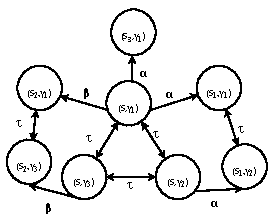
\includegraphics[width=\textwidth]{resources/st-before.pdf}
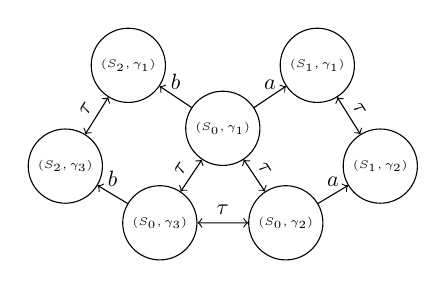
\begin{tikzpicture}[scale=.8, transform shape]		
\node[circle,draw] (n1) at (0,0) {\tiny$(S_0,\gamma_1)$};
\node[circle,draw] (n2) at (1,-1.5) {\tiny$(S_0,\gamma_2)$};
\node[circle,draw] (n3) at (-1,-1.5) {\tiny$(S_0,\gamma_3)$};
\node[circle,draw] (n4) at (1.5,1) {\tiny$(S_1,\gamma_1)$};
\node[circle,draw] (n5) at (2.5,-0.6) {\tiny$(S_1,\gamma_2)$};
\node[circle,draw] (n6) at (-1.5,1) {\tiny$(S_2,\gamma_1)$};
\node[circle,draw] (n7) at (-2.5,-0.6) {\tiny$(S_2,\gamma_3)$};
%\node[circle,draw] (n8) at (0,1.6) {\tiny$(S_3,\gamma_1)$};
\draw[<->]  (n1) edge node[above,sloped]{$\tau$} (n2);
\draw[<->]  (n1) edge node[above,sloped]{$\tau$} (n3);
\draw[<->]  (n2) edge node[above,sloped]{$\tau$} (n3);
\draw[<->]  (n5) edge node[above,sloped]{$\tau$} (n4);
\draw[<->]  (n6) edge node[above,sloped]{$\tau$} (n7);
%\draw[->]  (n1) edge node[right]{$a$} (n8);
\draw[->]  (n1) edge node[above]{$a$} (n4);
\draw[->]  (n1) edge node[above]{$b$} (n6);
\draw[->]  (n2) edge node[above]{$a$} (n5);
\draw[->]  (n3) edge node[above]{$b$} (n7);
\end{tikzpicture}
\caption{Before reduction}\label{Fig::stbefore}	
\end{subfigure}
\begin{subfigure}[b]{0.14\textwidth}
%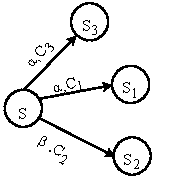
\includegraphics[width=\textwidth]{resources/st-after.pdf}
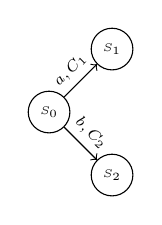
\begin{tikzpicture}[scale=.8, transform shape]			
\node[circle,draw] (n1) at (0,0) {\tiny$S_0$};
\node[circle,draw] (n2) at (1,1) {\tiny$S_1$};
\node[circle,draw] (n3) at (1,-1) {\tiny$S_2$};
%\node[circle,draw] (n4) at (1.5,0) {\tiny$S_3$};
\draw[->]  (n1) edge node[above,sloped]{\scriptsize$a,C_1$} (n2);
\draw[->]  (n1) edge node[above,sloped]{\scriptsize $b,C_2$} (n3);
%\draw[->]  (n1) edge node[above]{\scriptsize$a,C_3$} (n4);
\end{tikzpicture}
\caption{After reduction}\label{Fig::stafter}	
\end{subfigure}
\caption{A simple state space before and after applying the reduction. The network constraint $C_1$ expresses the common links of the topologies $\gamma_{1}$ and $\gamma_2$ while $C_2$ represents the common links of $\gamma_1$ and $\gamma_3$. %, and $C_3$ represents the links of $\gamma_1$.
}\label{Fig::reductionidea}	
\end{figure}

To tackle state-space explosion, we propose a symmetric reduction technique that eliminates the topology from the global states and combines those states that are only different in their topologies.  So the states $(S_0,\gamma_1)$, $(S_0,\gamma_2)$, and $(S_0,\gamma_3)$ of Figure \ref{Fig::stbefore} are aggregated to $S_0$ as demonstrated in Figure \ref{Fig::stafter}. As a consequence, transitions modifying the topology are removed (as they become self-loop $\tau$-transitions). 
A state transition like $S_0\overto{a} S_1$ is possible in Figure \ref{Fig::stafter} after the reduction, as we have $(S_0,\gamma_1)\overto{a}(S_1,\gamma_1)$ and $(S_0,\gamma_2)\overto{a}(S_1,\gamma_2)$ in Figure \ref{Fig::stbefore} before the reduction. In other words, when the local states of rebecs is $S_0$ and the underlying topology is either $\gamma_1$ or $\gamma_2$, handling the same message, represented by $a$, leads to the same next local states, i.e., $S_1$.  As message handlers are executed with regard to the topology, the connectivity/disconnectivity of those links that are common in both topologies make the effect of handling the message to be the same. The connectivity/disconnectivity relations of these links, called \emph{network constraint}~\cite{FatemehFI10,FatemehFI19},  are added to the labels on the transitions. For example, the links common in both $\gamma_{1}$ and $\gamma_{2}$ that result in the same next local states, i.e., $S_1$ in Figure \ref{Fig::stbefore}, are added by the network constraint $C_1$ to the label of the transition $S_0\overto{a,C_1}S_1$ in Figure \ref{Fig::stafter}. %For instance, the network constraint ${\it and}({\it con}(n_1,n_2),!{\it con}(n_3,n_4))$ expresses that the actor  $n_1$ is connected to $n_2$ while $n_3$ is disconnected from $n_4$. 
To enforce a set of stable connectivity/disconnectivity relations among the actors, we specify them by a network constraint at the \emph{constraints} block of the model. For instance, the network constraint given in line $68$ of Figure \ref{code:aodv} enforces $n_3$ to be always connected to $n_4$, expressed by ${\it con}(n_3,n_4)$.  
%Our reduction technique is indeed a form of symmetric reduction technique \cite{clarke1998symmetry}. 
As this reduction technique is applied at the transition system level, it can be also applied if the actors were not isolated. However, the non-preemptive execution of event handlers at the model level makes this reduction at the state-space level more effective for the analysis of real-world protocols like AODV. 


\fixme{Here you are talking only about the "atomic execution of methods", right? that we cannot really call isolation ... we should talk about atomic execution of methods and then maybe say why we can do it without loss of generality, that is because of isolation.}
In following we discuss the amount of reductions achieved by combination of the isolation at the model
level and topology elimination at the level of the transition system. The topology-elimination reduction technique eliminates the topology $\gamma$ from the global state $(S,\gamma)$ and generates the next local actor states for handling messages
considering all possible connectivity/disconnectivity of the handling actor to other actors. For a network of $n$ nodes, each node has $2^{n-1}$ possible connectivity/disconnectivity relations with others. So, the topology-elimination reduction technique reduces the number of states from $\mathbb{S}\times 2^{(n^2-n)}$ to $\mathbb{S}\times2^{n-1}$, where $\mathbb{S}$ is the total number of possible local states of actors. If $\mathbb{S}$ be a large number, the reduction achieved by topology-elimination is not sufficient enough for tackling state-space explosion, as we experienced in the algebraic framework of \cite{FORM}. If message handlers were preemptive, $\mathbb{S}$ would be indeed huge because of enormous possible interleaving of message handlers. Restricting to isolated actors, minimizes $\mathbb{S}$ substantially. 
%
%
%Assume a snapshot of a model where we have $k$ actors that each has at least one event in its queue to handle, and the corresponding event handlers of events have $i_1$, $\ldots$, $i_k$ statements in the model. 
%\Fatem{why you have k actors, and also k statements?}
%When actors are not isolated, the local states of actors are defined by triple elements in the micro-step semantics: state variable valuation, queue contents, and the pointer to the statements to be executed (PC). For handling these $k$ events, $m\times 2^{(n^2-n)}$ global states are generated at the micro-step semantic level, where $m$ is the number of possible interleaving of event handler's statements (hence, the number of possible local states). The topology-elimination reduction technique reduces the number of states from $m\times 2^{(n^2-n)}$ to $m\times2^{n-1}$. If $m$ be a large number, the reduction achieved by topology-elimination is not sufficient enough for tackling state-space explosion, as we experienced in the algebraic framework of \cite{FORM}. Restricting to isolated actors, minimizes $m$ substantially.
%
%\fixme{maybe we remove computing of m, remove the following paragraph?}
%We compute $m$ to show that it is indeed large. As there are $i_1+\ldots+i_k$ slots for the statements, we choose $i_1$ in which to place the first event handler statements, $i_2$ of the remaining slots in which to place the second event handler instructions, and so on. This gives the result  ${\small m=\begin{pmatrix}
%	%\displaystyle\sum_{j=1}^{k} i_j \\
%	i_1+\ldots+i_k\\
%	i_1 \\
%	\end{pmatrix}\times
%	\begin{pmatrix}
%	%\displaystyle\sum_{j=2}^{k} i_j \\
%	i_2+\ldots+i_k\\
%	i_2 \\
%	\end{pmatrix}\times	\ldots\times
%	\begin{pmatrix}
%	%\displaystyle\sum_{j=k}^{k} i_j \\
%	i_k\\
%	i_k \\
%	\end{pmatrix}}$ which equals to ${\small %\frac
%{(\sum_{j=1}^{k} i_j)!}/{\prod_{j=1}^{k}(i_j!)}.}$ 
%Restricting to isolated actors, minimizes $m$ substantially to $k!$. The combination of isolation at the model and topology-elimination reduction approach at the semantics shrinks the state space substantially for real-world protocols and hence, makes the model checking technique possible as shown in Table \ref{Tab:aodv-redu}. 
%
Table \ref{Tab:aodv-redu} illustrates the amount of reduction achieved by applying topology-elimination reduction on isolated actors. When the number of nodes increases from $4$ to $5$ for AODV while the specified network constraint at the model results only $16$ possible topologies, the state space cannot be generated due to the memory limitation on a computer with $8${GB} {RAM}.  We proved that the reduced state space is branching bisimilar to the
original one, and consequently a set of properties such as {ACTL-X} are preserved \cite{FOAC}. The network constraints on transition are used during model checking \cite{FORM,CSI2018} to verify the topology-sensitive properties. 

\begin{table*}
	%   \renewcommand{\arraystretch}{1.5}
	\centering
	\caption{Comparing the size of state spaces with/without applying reduction \cite{FOAC}}
	\begin{tabular*}{0.75\textwidth}{@{\extracolsep{\fill }} |   c  c  r  r  r  r  |   }
		\hline
		No. of & No. of valid & No. of states    &  No. of transitions     & No. of states & No. of transitions
		\\
		nodes & topologies & before reduction  &  before reduction   & after reduction &  after reduction
		\\
		\hline	     
		4 & 4 & 3,007 & 16,380 & 763  & 1,969 \\
		4  & 8 & 12,327 & 113,480 & 1,554  & 3,804 \\
		4  & 16 & 35,695 & 610,816 & 2,245 & 5,549 \\    
		4  & 32 & 93,679 & 3,097,792 & 2,942 & 7,596 \\  
		4    & 64  & 258,447  & 16,797,536 & 4,053 & 10,629 \\
		5 & 16 & $>$655,441 & $>$11,276,879 & 165,959 &  598,342 \\
		\hline
	\end{tabular*}
	\label{Tab:aodv-redu}
\end{table*}

